% Este trabalho está licenciado sob a licença Creative Commons CC-BY-SA.
% Você é livre para usar, compartilhar e adaptar este material, desde que seja atribuída a autoria e que as obras derivadas mantenham a mesma licença.

%-----------------------------Apêndices-----------------------------%
\begin{apendicesenv}


\chapter{Tutorial de uso do modelo LaTeX de monografia/dissertação/tese PUCPR}
\label{apendice_tutorial}

Este modelo foi desenvolvido pelos professores Rayson Laroca e Jean Paul Barddal em \LaTeX, tomando como base um modelo de dissertação da Universidade Federal do Tocantins (UFT) estruturado com a classe \abnTeX.
Foram realizadas diversas adaptações para garantir sua conformidade com as normas para elaboração de trabalhos acadêmico-científicos da Pontifícia Universidade Católica do Paraná (PUCPR), que, por sua vez, seguem as diretrizes da Associação Brasileira de Normas Técnicas (ABNT).

\section*{1. Apresentação do Modelo}

Neste tutorial, será apresentada a estrutura básica do modelo a fim de facilitar sua utilização.
O modelo está disponível no seguinte endereço eletrônico: \url{https://www.overleaf.com/read/nqpnfkmqzhkb\#40fc88}.
Ao abrir o link em sua conta Overleaf, o usuário terá acesso a uma tela semelhante à mostrada na Figura\ref{fig:estrutura}.

\begin{figura}{0.9\textwidth}
    \caption{Modelo aberto no editor online Overleaf.}
    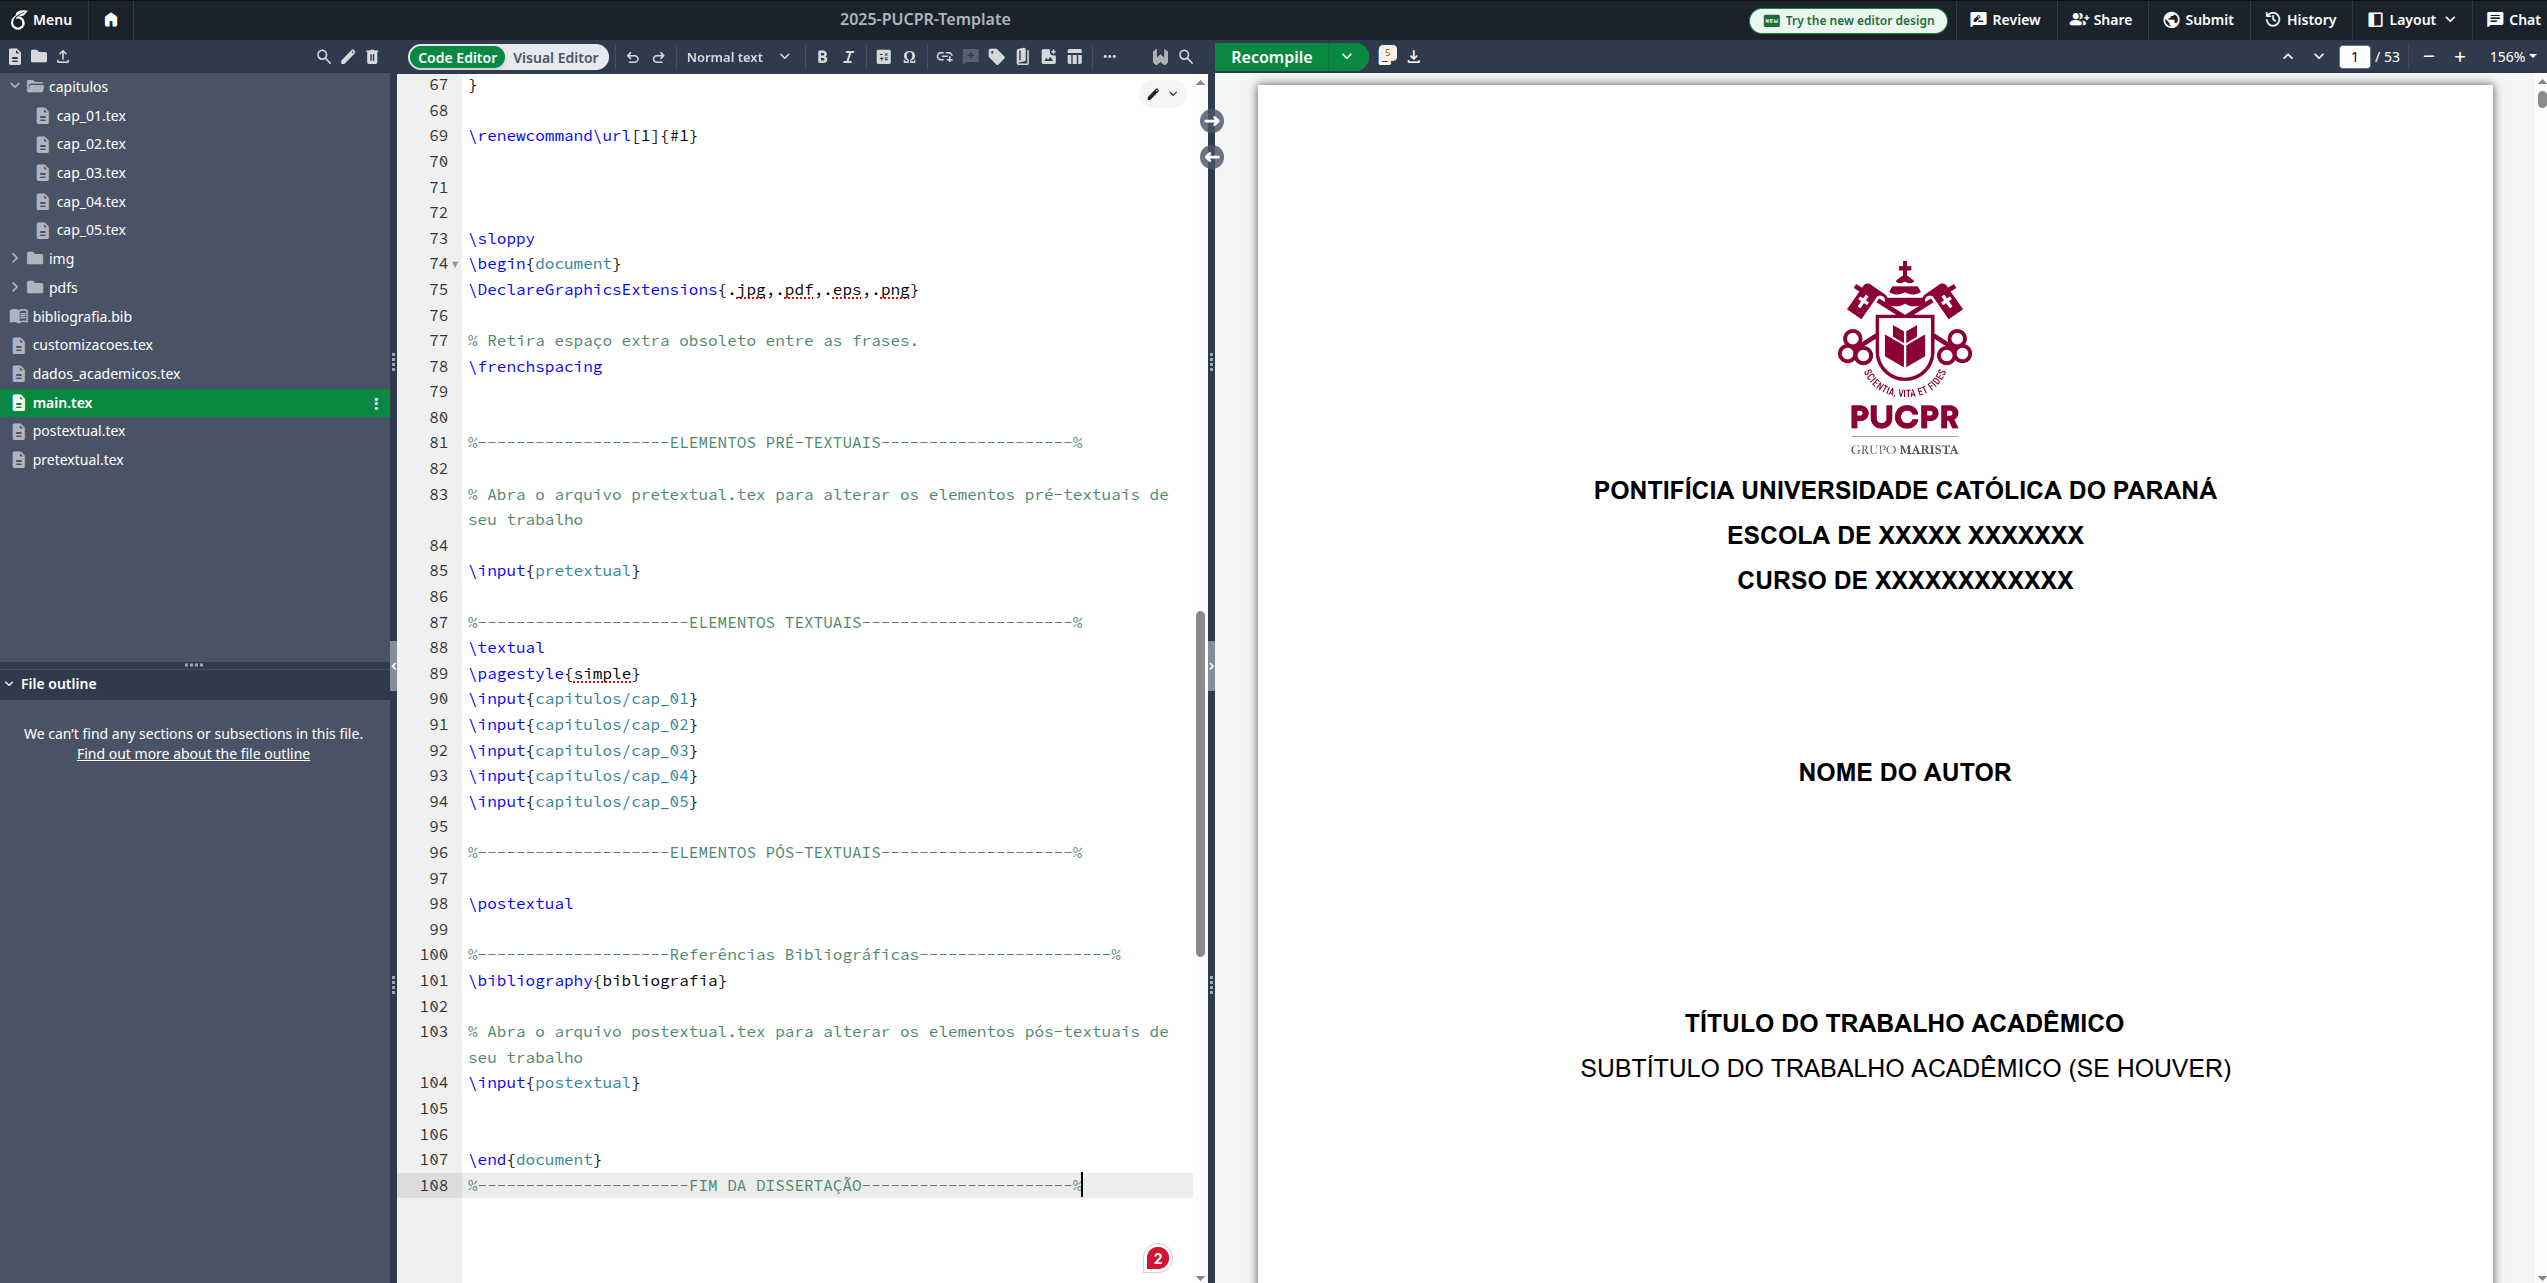
\includegraphics[width=\textwidth]{img/modelo/estrutura_arquivos.png}
    \label{fig:estrutura}
    \sourceFig{o autor, 2025.}
\end{figura}


A imagem mostra uma interface de um editor de LaTeX online  Overleaf. O editor está dividido em três seções:  Na coluna da esquerda encontra-se a estrutura de arquivos de um projeto de dissertação, com destaque para o arquivo principal: \verb|main.tex|. A coluna central mostra o documento atualmente aberto (nesse caso, o código-fonte do arquivo \verb|main.tex|). Por fim, a coluna direita apresenta uma visualização prévia do arquivo PDF produzido. 

A estrutura de arquivos da coluna esquerda é resumida a seguir:
    \begin{itemize}
        \item \verb|capitulos/|: Pasta contendo os arquivos dos capítulos do documento (\verb|cap_01.tex|, \verb|cap_02.tex|, etc.).
        \item \verb|img/|: Pasta para armazenar imagens, embora esteja colapsada e não possamos ver o conteúdo.
        \item \verb|pdfs/|: Pasta contendo vários PDFs, como anexos e apêndices (\verb|anexo_exemplo.pdf|, \verb|anexo_latex_symbols.pdf|, etc.).
        \item \verb|bibliografia.bib|: Arquivo BibTeX contendo referências bibliográficas.
        \item \verb|customizacoes.tex|: Arquivo contendo customizações específicas para o projeto.
        \item \verb|dados_academicos.tex|: Arquivo contendo informações acadêmicas (autor, título, orientador, etc.).
        \item \verb|main.tex|: Arquivo principal do documento LaTeX. É aconselhado que esteja com esse arquivo aberto sempre que necessitar \textbf{recompilar} seu projeto.
        \item \verb|postextual.tex| e \verb|pretextual.tex|: Arquivos para as partes pré-textuais e pós-textuais do documento.
    \end{itemize}

Nas seções seguintes, apresentamos uma sugestão de sequência de preenchimento do modelo para o desenvolvimento do seu documento.

\section*{2. Dados Acadêmicos}

Abra o arquivo \verb|dados_academicos.tex| e preencha as os campos referentes ao título do trabalho, subtítulo (caso não haja subtítulo, basta apagar (comentar) a linha correspondente a esse campo), autor, orientador, instituição, câmpus e data. A Figura \ref{fig:dados-academicos} ilustra um exemplo de preenchimento com dados~fictícios.

\begin{figura}{0.9\textwidth}
    \caption{Preenchimento dos dados acadêmicos.}
    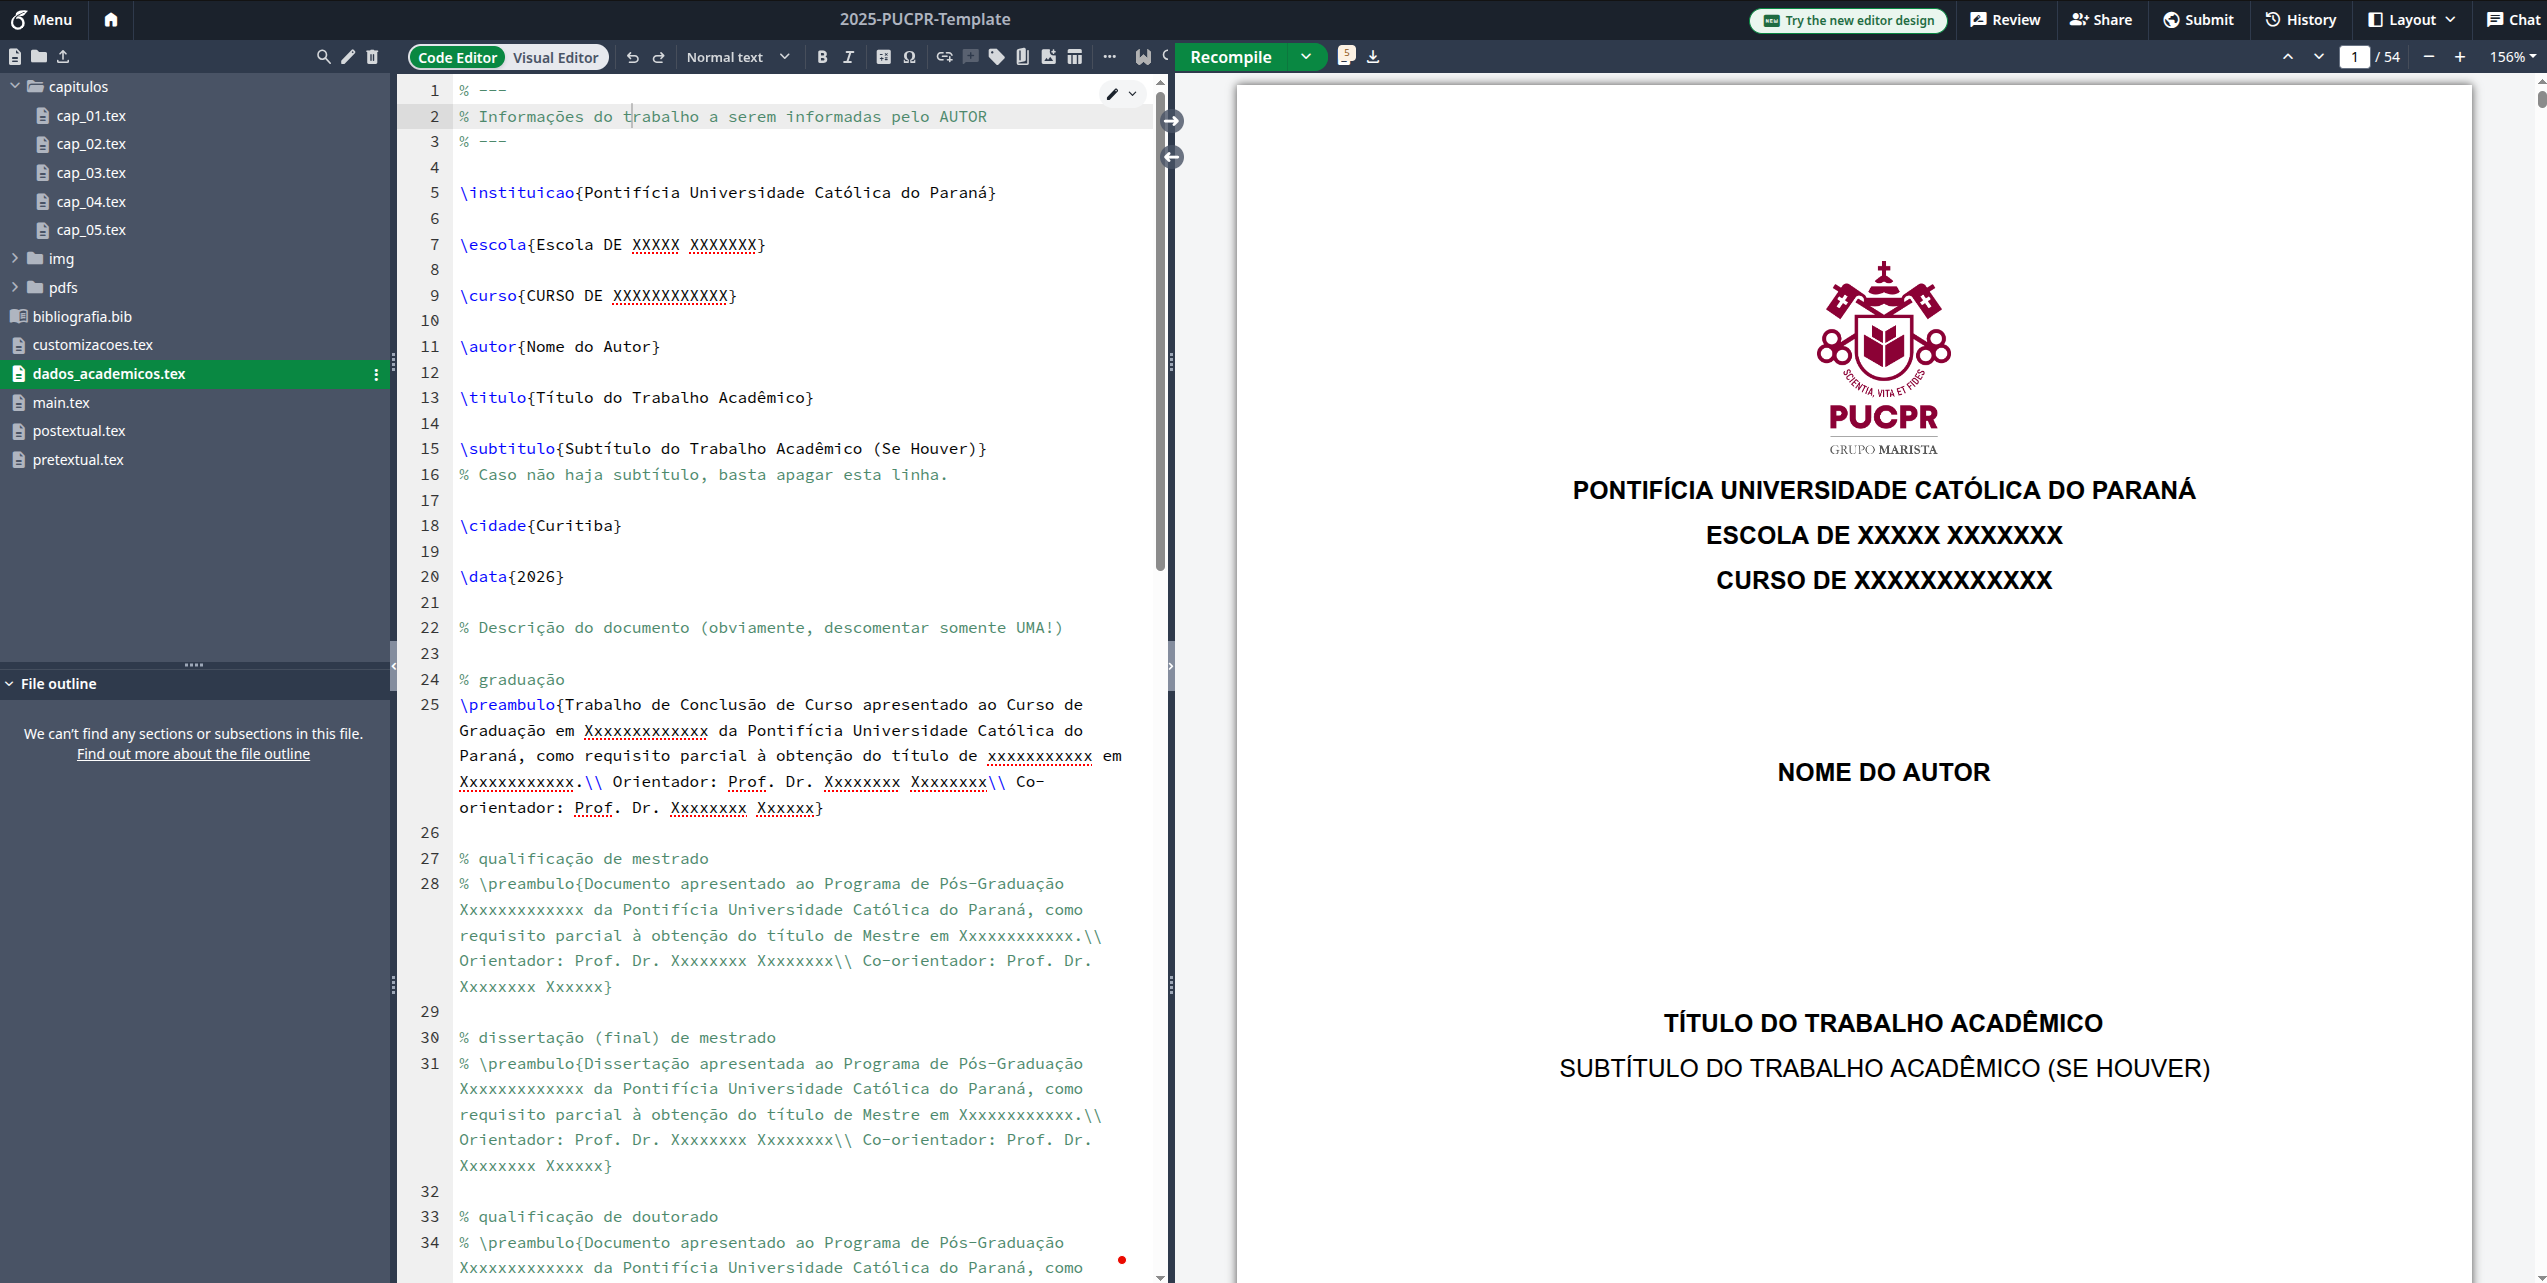
\includegraphics[width=\textwidth]{img/modelo/dados_academicos.png}
    \label{fig:dados-academicos}
    \sourceFig{o autor, 2025.}
\end{figura}

Ao clicar no botão \textbf{recompilar} do editor, os dados informados serão automaticamente carregados nos campos correspondentes tanto da capa quanto na folha de rosto do trabalho.

\section*{3. Elementos pré-textuais}

Os elementos pré-textuais são as partes iniciais de um trabalho acadêmico que antecedem o conteúdo principal. Eles são fundamentais para a estrutura e apresentação do documento, fornecendo informações essenciais sobre o trabalho, seus autores e orientadores, bem como a instituição\footnote{Para mais detalhes sobre os elementos pré-textuais (obrigatórios e opcionais), leia a norma ABNT NBR 14724 \cite{nbr14724}}.

Abra o arquivo \verb|pretextual.tex|. A seguir, mostra-se o preenchimento das principais informações pré-textuais.

A Figura \ref{fig:pretextual-01} mostra os primeiros quatro elementos pré-textuais: Capa, Folha de Rosto, Ficha Catalográfica e Folha de Aprovação. Quanto aos dois primeiros, nenhuma intervenção é necessário pois são elementos de formatação padronizada cujos dados foram informados no arquivo \verb|dados_academicos.tex| como detalhado na seção anterior.

\begin{figura}{0.9\textwidth}
    \caption{Elementos pré-textuais: Ficha catalográfica e Folha de aprovação.}
    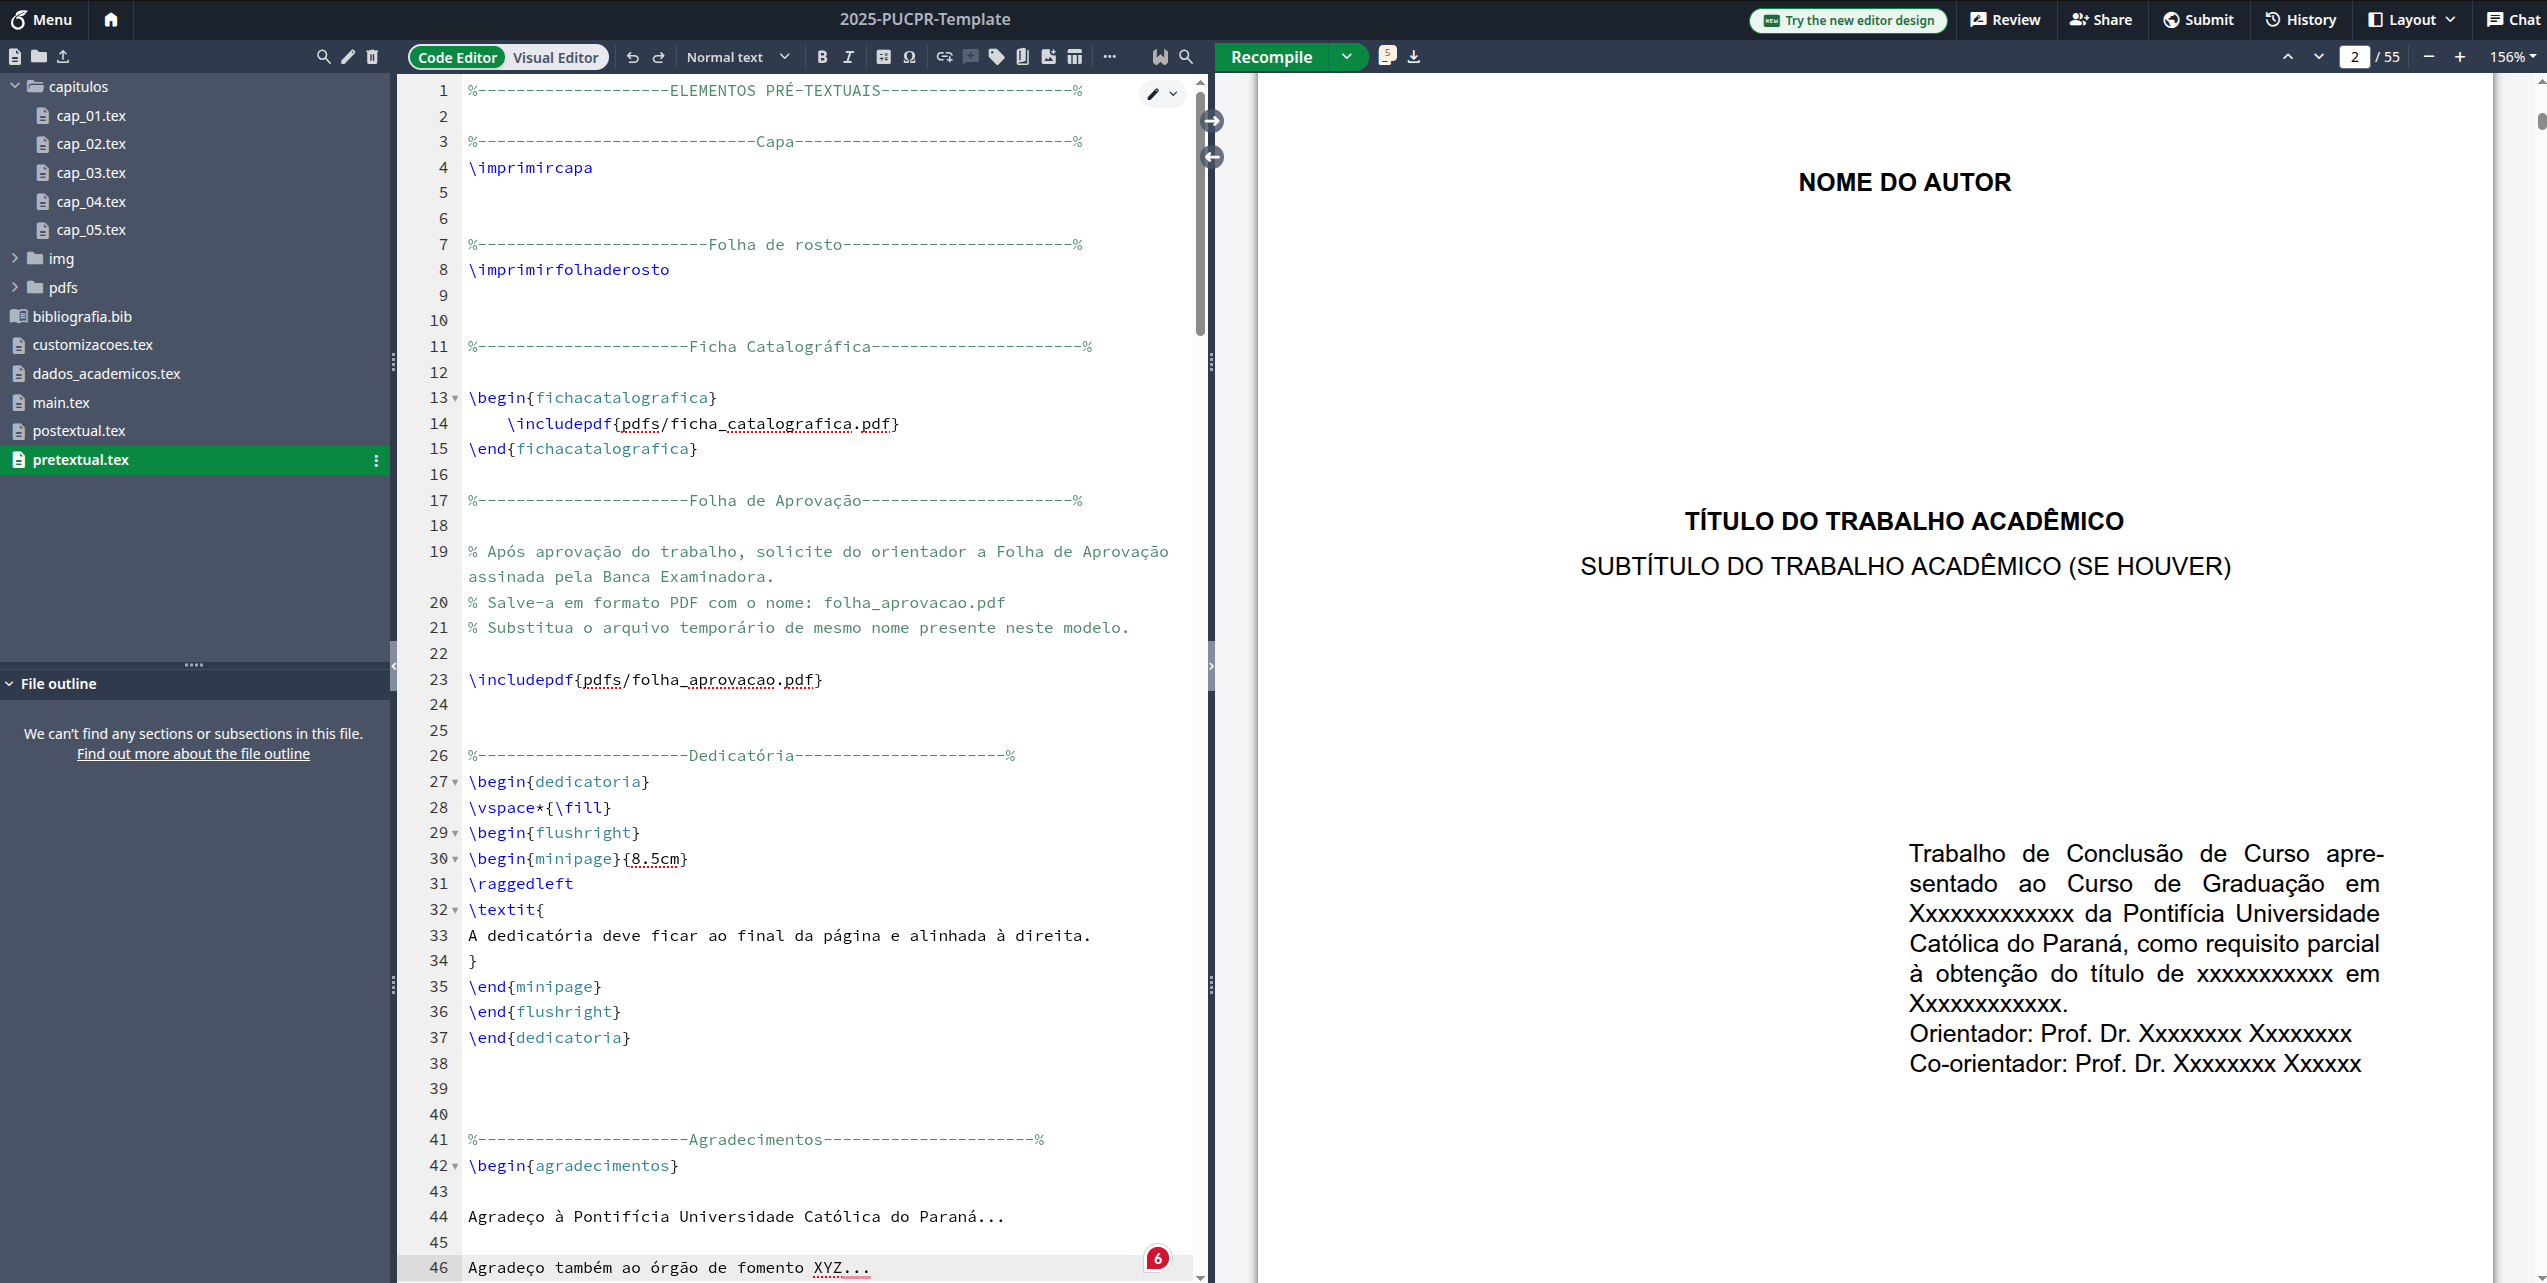
\includegraphics[width=\textwidth]{img/modelo/pretextual-01.png}
    \label{fig:pretextual-01}
    \sourceFig{o autor, 2025.}
\end{figura}

A respeito da Ficha Catalográfica e da Folha de Aprovação, tratam-se de documentos cujo preenchimento ocorrerá após a aprovação do trabalho e as correções sugeridas pela Banca Examinadora.

\subsection*{3.1 Ficha Catalográfica}
Após a aprovação do trabalho, faça o download da ficha em formato PDF e salve-a com o nome: \verb|ficha_catalografica.pdf| dentro da pasta \verb|pdfs|. 

\subsection*{3.2 Folha de Aprovação}

Após aprovação do trabalho, solicite ao orientador a Folha de Aprovação assinada pela Banca Examinadora. Salve-a em formato PDF com o nome: \verb|folha_aprovacao.pdf|. Substitua o arquivo temporário de mesmo nome presente na pasta \verb|pdfs| neste modelo.


Nos dois casos acima, esteja atento para o correto nome de arquivos, bem como o local em que devem ser salvos. Ao clicar em \textbf{Recompilar}, os novos arquivos serão carregados em seu trabalho.

Os próximos elementos pré-textuais são: Dedicatória, Agradecimentos e Epígrafe. Seu preenchimento é bastante intuitivo, conforme mostrado na Figura \ref{fig:pretextual-02}.

\begin{figura}{0.9\textwidth}
    \caption{Elementos pré-textuais: Dedicatória, Agradecimentos e Epígrafe.}
    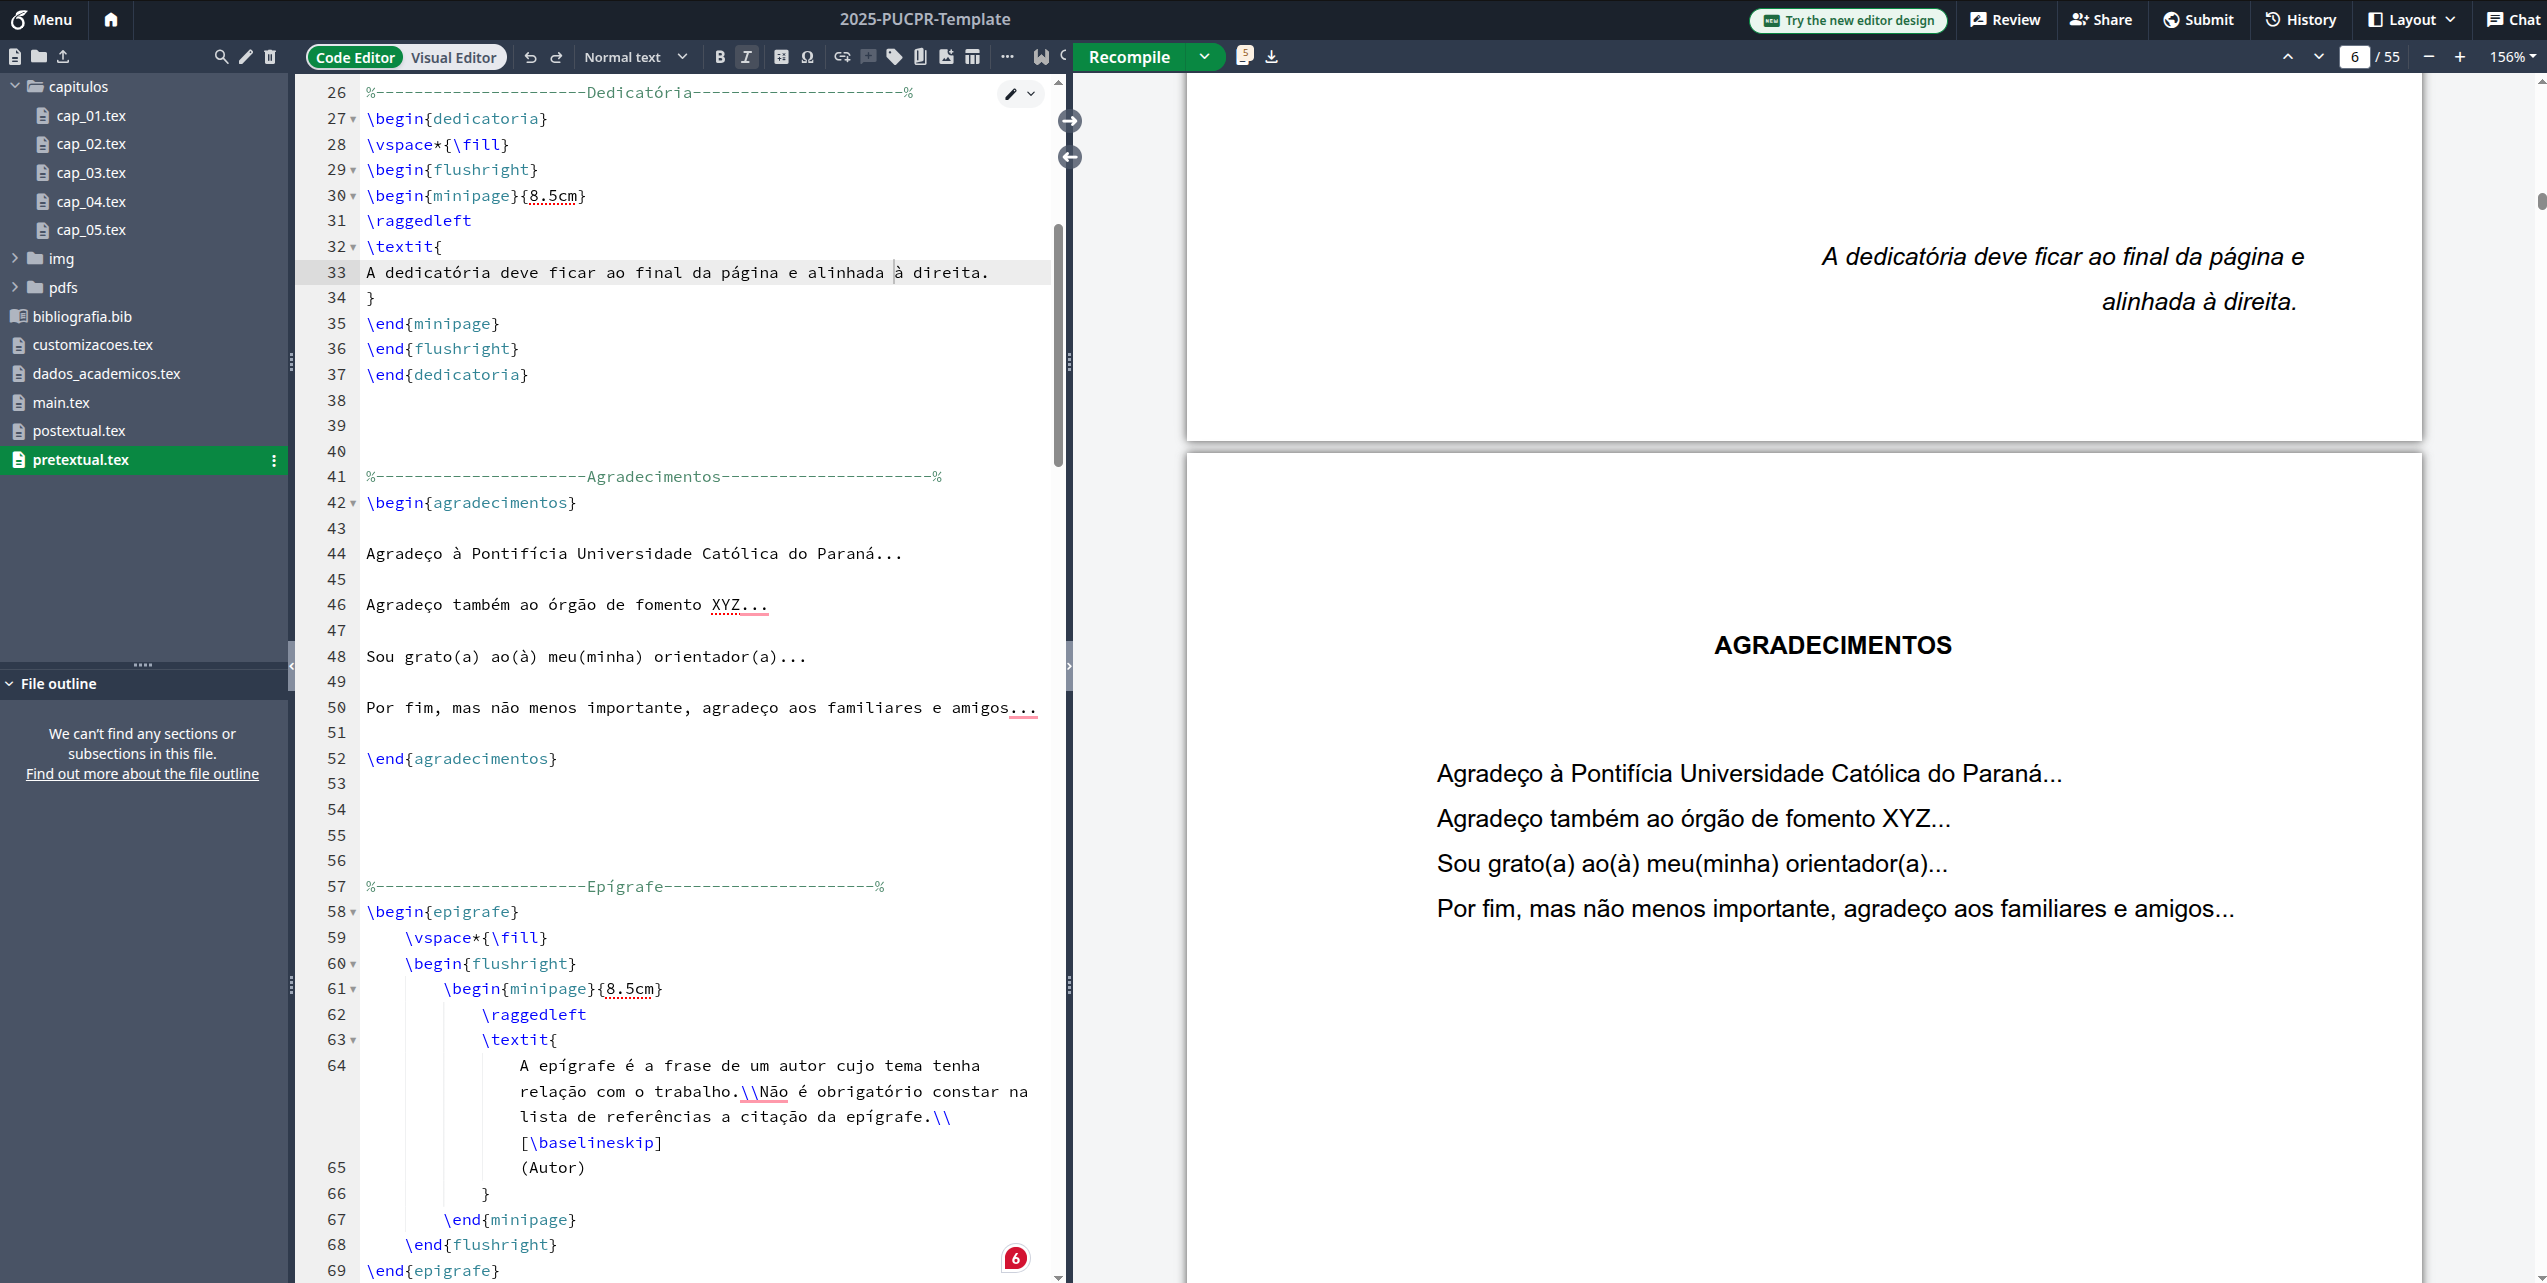
\includegraphics[width=\textwidth]{img/modelo/pretextual-02.png}
    \label{fig:pretextual-02}
    \sourceFig{o autor, 2025.}
\end{figura}


Em seguida, tem-se o resumo (em língua portuguesa e em língua estrangeira), conforme mostrado na Figura \ref{fig:pretextual-03}. Observe que de acordo com a norma ABNT NBR 6028:2021 o resumo deve apresentar o conteúdo do trabalho de  forma sucinta, composto por uma sequência de frases concisas em parágrafo único, sem enumeração de tópicos e escritas com verbo na terceira pessoa \cite{nbr6028}.

\begin{figura}{0.9\textwidth}
    \caption{Elementos pré-textuais: Resumo e Abstract.}
    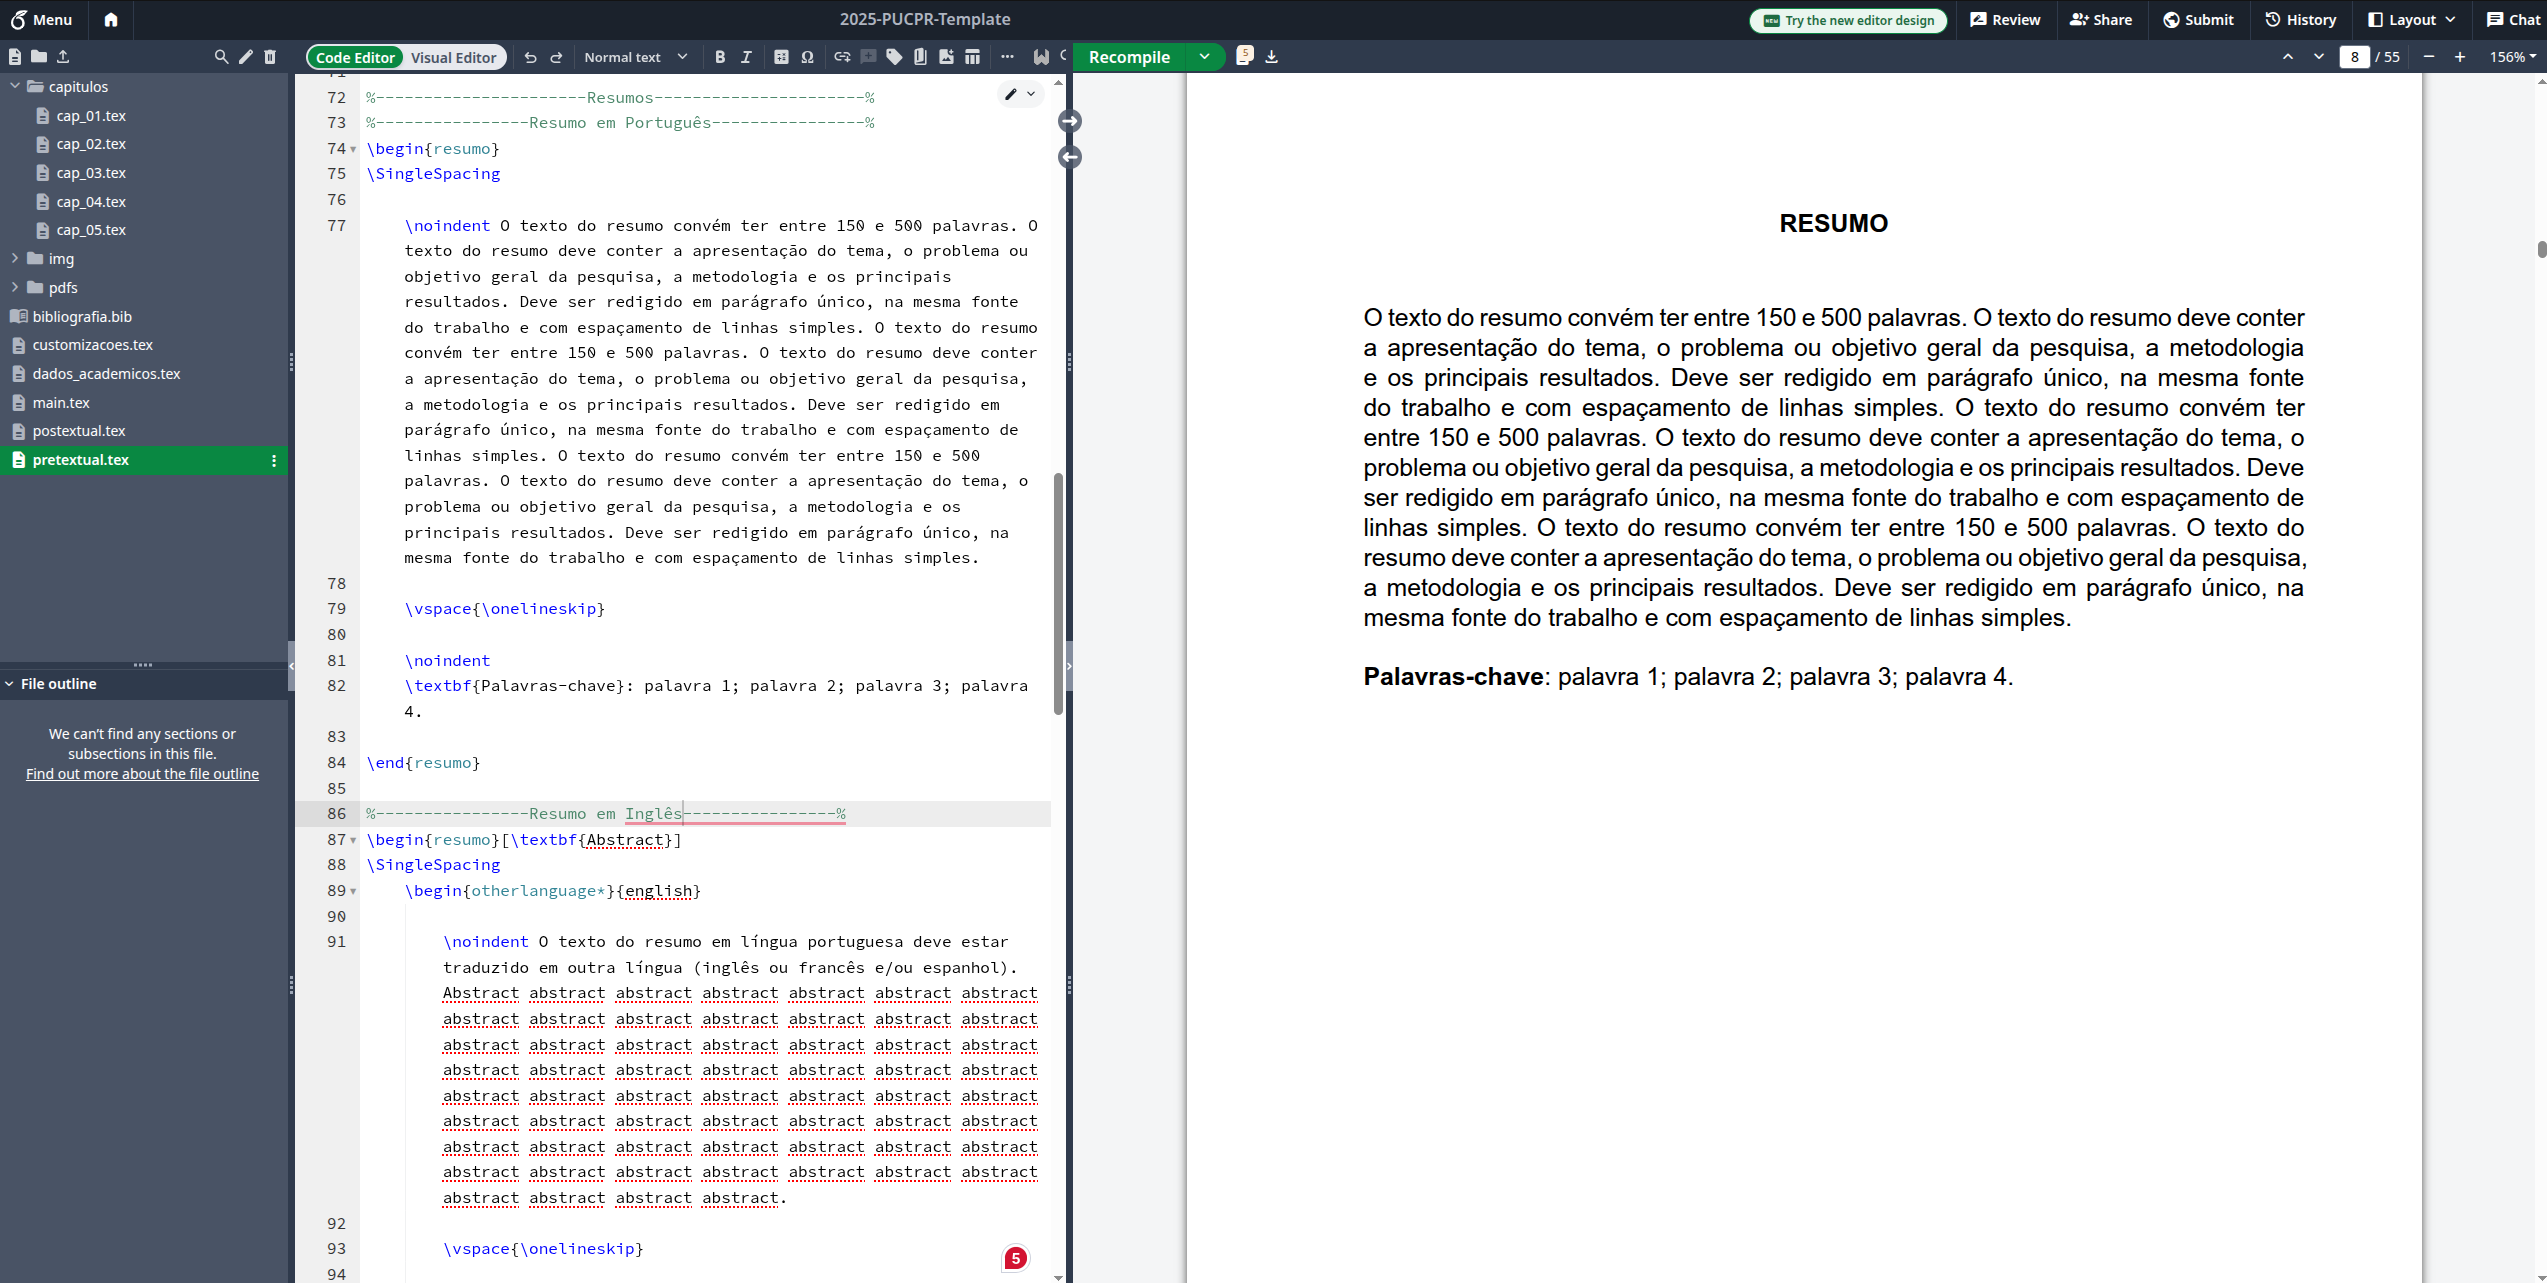
\includegraphics[width=\textwidth]{img/modelo/pretextual-03.png}
    \label{fig:pretextual-03}
    \sourceFig{o autor, 2025.}
\end{figura}

Quanto às palavras-chave, segundo a norma ABNT NBR 6028:2021, devem ser separadas entre si por ponto e vírgula e finalizadas por ponto.  A referida norma ainda ressalta que as palavras-chave devem ser grafadas com iniciais em letras minúsculas, exceto quando substantivos próprios e nomes científicos \cite{nbr6028}.

Uma importante parte  dos elementos pré-textuais são as listas. A Figura \ref{fig:pretextual-04} mostra as listas de ilustrações, quadros, tabelas, abreviaturas e siglas e símbolos.


\begin{figura}{0.9\textwidth}
    \caption{Elementos pré-textuais: Listas.}
    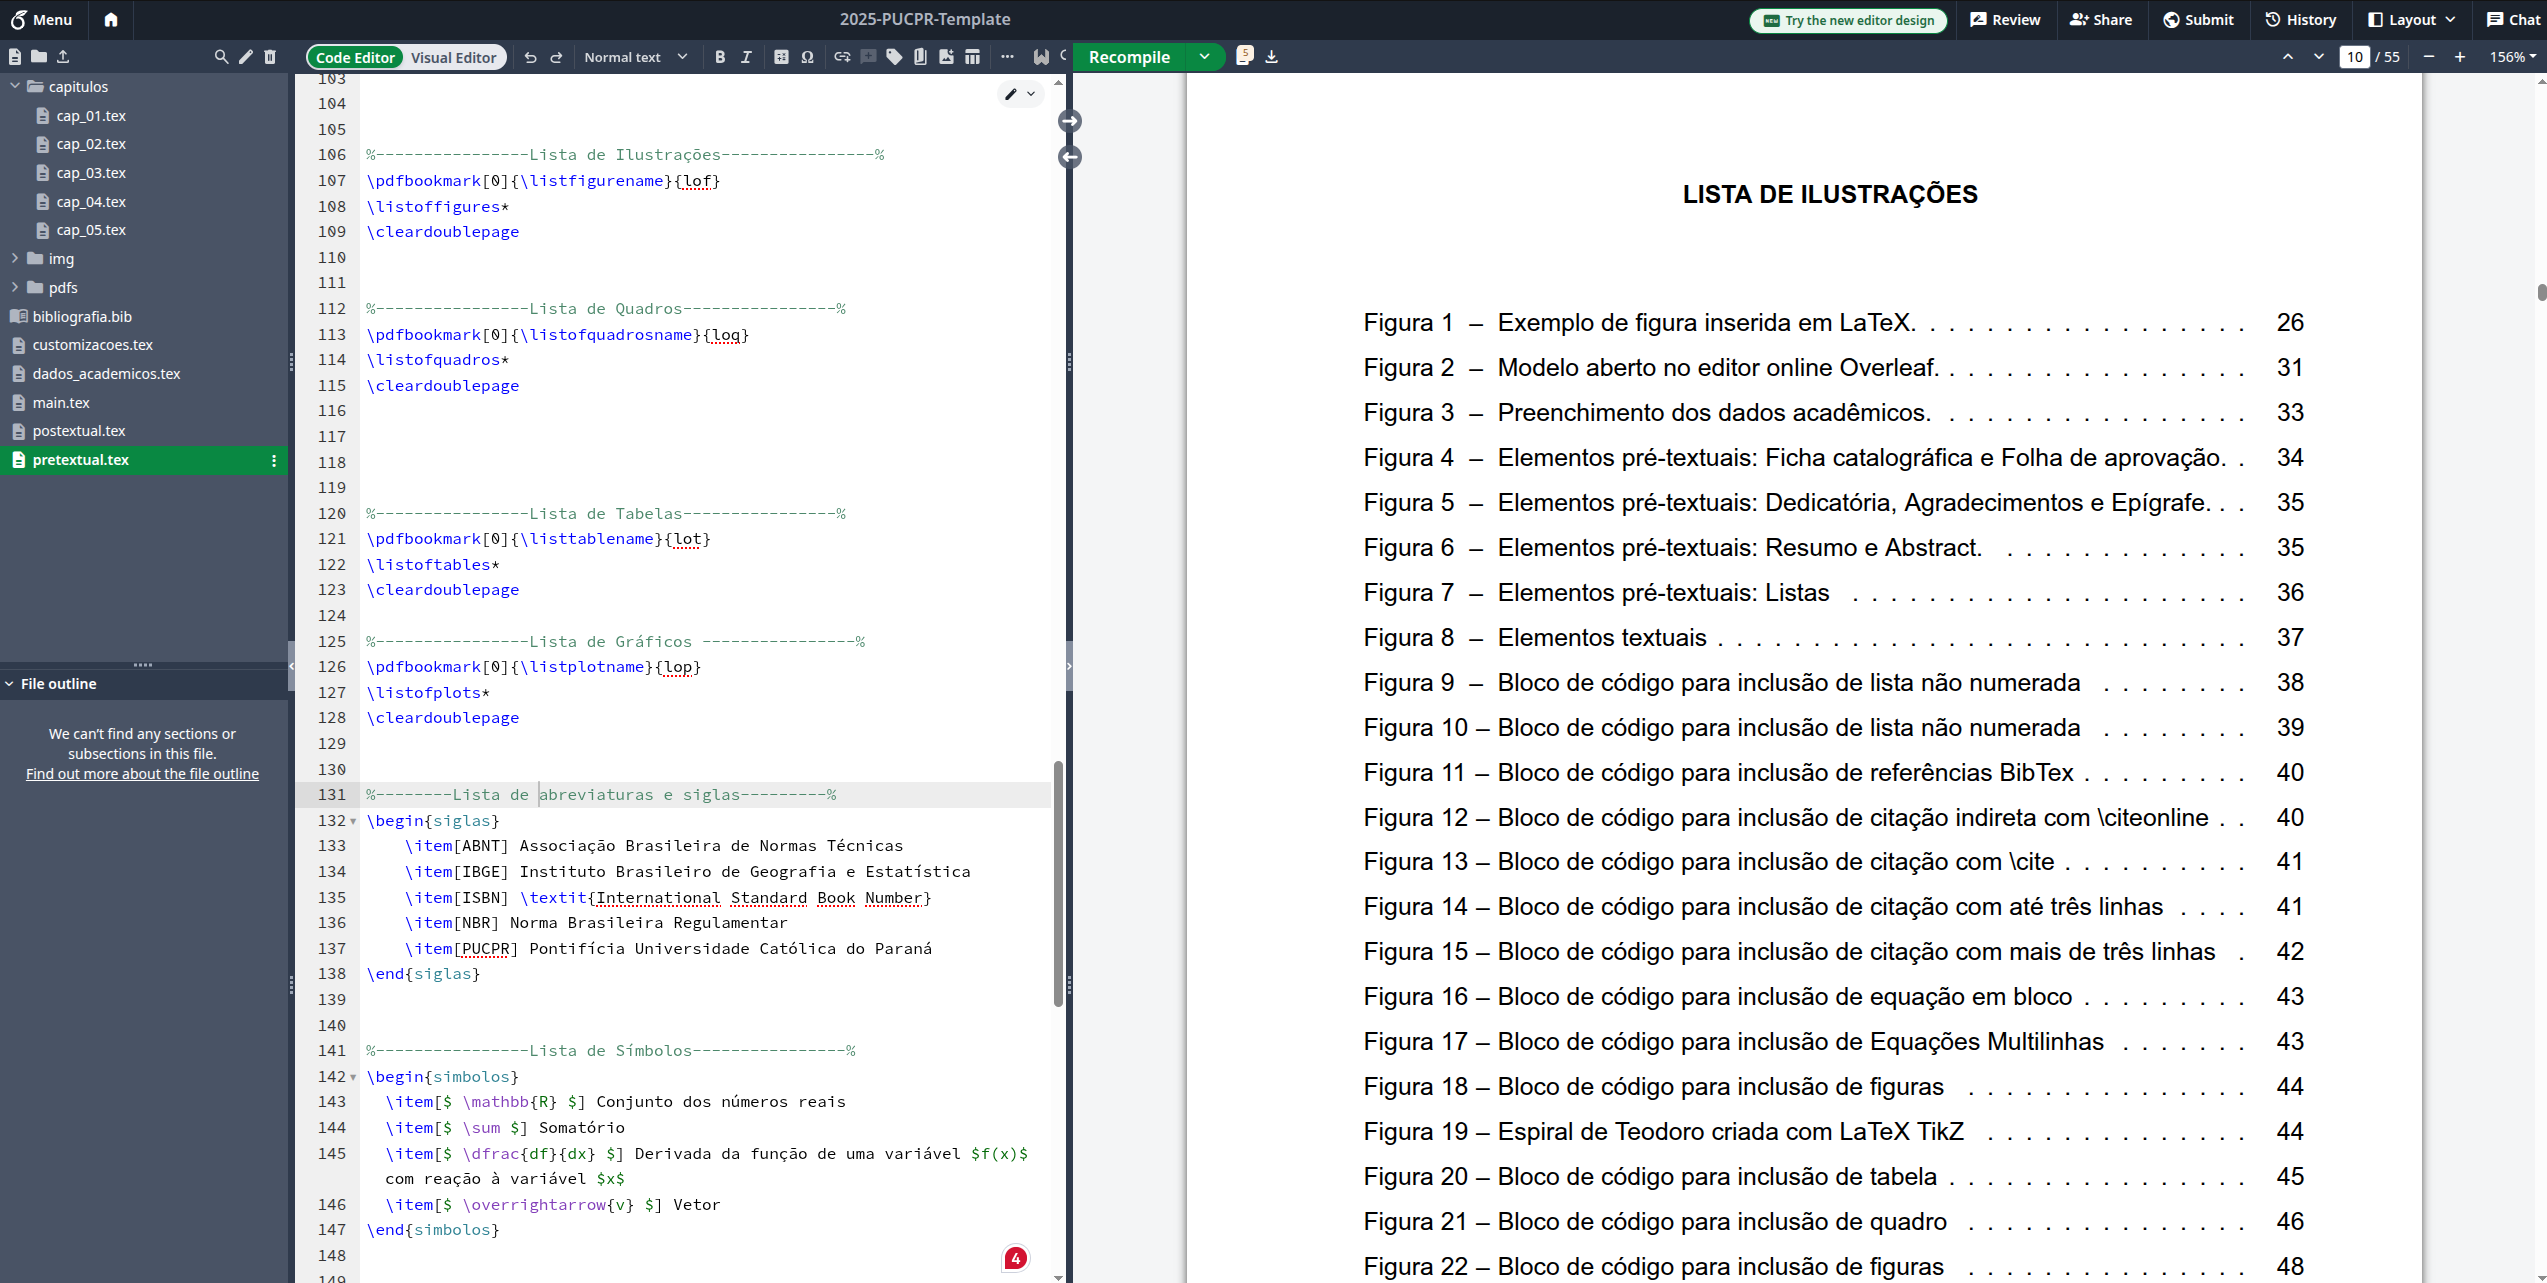
\includegraphics[width=\textwidth]{img/modelo/pretextual-04.png}
    \label{fig:pretextual-04}
    \sourceFig{o autor, 2025.}
\end{figura}

Observe que a Listas de Ilustrações, a Lista de Quadros e a Lista de Tabelas são criadas automaticamente, à medida que estes elementos são incluídos no texto do trabalho. Portanto, apenas a Lista de Abreviaturas e Siglas  e a Lista de Símbolos requerem preenchimento manual pelo autor do trabalho. Alguns exemplos podem ser encontrados no arquivo \verb|pretextual.tex|.

Para finalizar a parte de elementos pré-textuais, tem-se o sumário. À  medida que o autor adiciona novos capítulos (\verb|\chapter{|), seções (\verb|\section|) e subseções (\verb|\subsection|), o sumário será atualizado automaticamente.

\section*{4. Elementos Textuais}

Para uma melhor organização do trabalho, a parte textual do documento foi dividida em capítulos: \verb|cap_01.tex|, \verb|cap_02.tex|, \verb|cap_03.tex|, \verb|cap_04.tex| e \verb|cap_05.tex| dentro na pasta \verb|capitulos|.  Note que o carregamento desses arquivos para a dissertação é feito por meio do comando \verb|\input| no arquivo principal \verb|main.tex|, como mostrado na Figura \ref{fig:textual-01}.

\begin{figura}{0.9\textwidth}
    \caption{Elementos textuais.}
    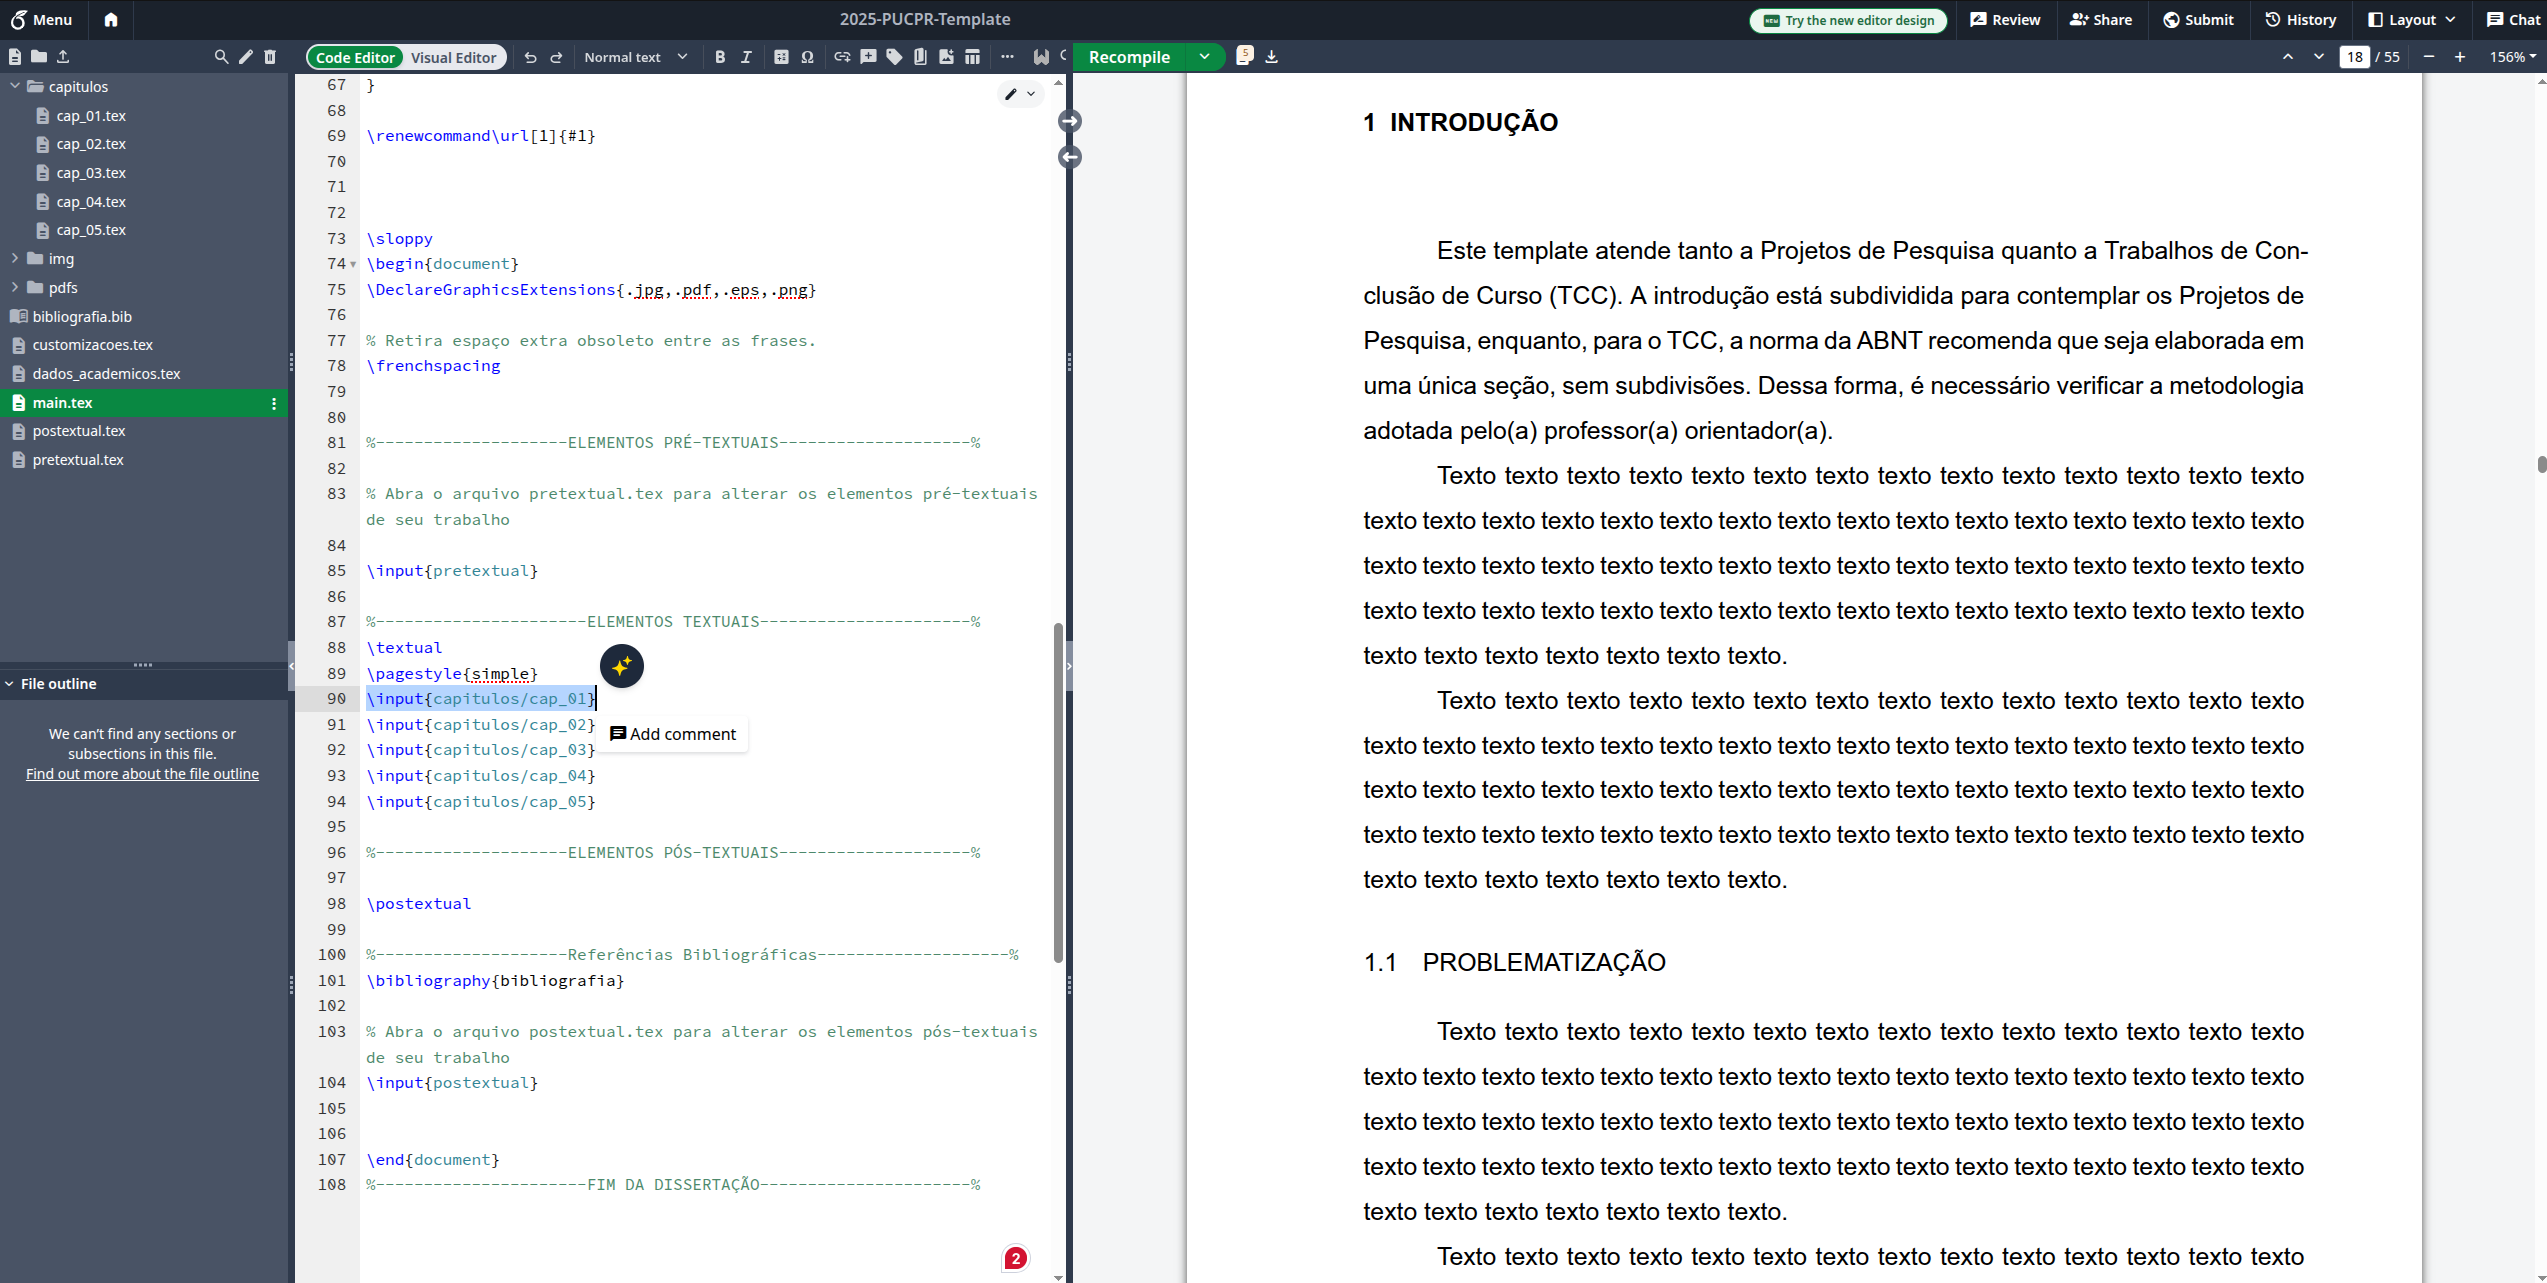
\includegraphics[width=\textwidth]{img/modelo/textual-01.png}
    \label{fig:textual-01}
    \sourceFig{o autor, 2025.}
\end{figura}

Observe na Figura \ref{fig:textual-01} que para a inclusão do arquivo \verb|cap_01.tex| foi utilizado o comando \verb|%----------------Cap_01----------------%

\chapter{Introdução}

Este modelo atende tanto a projetos de pesquisa quanto a Trabalhos de Conclusão de Curso~(TCC).
A introdução está subdividida para contemplar os Projetos de Pesquisa, enquanto, para o TCC, a norma da ABNT recomenda que seja elaborada em uma única seção, sem subdivisões.
Dessa forma, é necessário verificar a metodologia adotada pelo(a) professor(a) orientador(a).

Um tutorial de uso do modelo está disponível no Apêndice~\ref{apendice_tutorial}.

Texto texto texto texto texto texto texto texto texto texto texto texto texto texto texto texto texto texto texto texto texto texto texto texto texto texto texto texto texto texto texto texto texto texto texto texto texto texto texto texto texto texto texto texto texto texto texto texto texto texto texto texto texto texto texto texto texto texto texto texto texto texto texto texto texto texto texto texto texto.

Texto texto texto texto texto texto texto texto texto texto texto texto texto texto texto texto texto texto texto texto texto texto texto texto texto texto texto texto texto texto texto texto texto texto texto texto texto texto texto texto texto texto texto texto texto texto texto texto texto texto texto texto texto texto texto texto texto texto texto texto texto texto texto texto texto texto texto texto texto.

\section{Problematização}

Texto texto texto texto texto texto texto texto texto texto texto texto texto texto texto texto texto texto texto texto texto texto texto texto texto texto texto texto texto texto texto texto texto texto texto texto texto texto texto texto texto texto texto texto texto texto texto texto texto texto texto texto texto texto texto texto texto texto texto texto texto texto texto texto texto texto texto texto texto.

Texto texto texto texto texto texto texto texto texto texto texto texto texto texto texto texto texto texto texto texto texto texto texto texto texto texto texto texto texto texto texto texto texto texto texto texto texto texto texto texto texto texto texto texto texto texto texto texto texto texto texto texto texto texto texto texto texto texto texto texto texto texto texto texto texto texto texto texto texto.

De acordo com \cite{gil2008metodos}:

\begin{citacao}
    citação citação citação citação citação citação citação citação citação citação citação citação citação citação citação citação citação citação citação citação citação citação. Citação citação citação citação citação citação citação citação citação citação citação citação citação citação citação citação citação citação citação citação citação citação.
\end{citacao}

Texto texto texto texto texto texto texto texto texto texto texto texto texto texto texto texto texto texto texto texto texto texto texto texto texto texto texto texto texto texto texto texto texto texto texto texto texto texto texto texto texto texto texto texto texto texto texto texto texto texto texto texto texto texto texto texto texto texto texto texto texto texto texto texto texto texto texto texto texto.

Texto texto texto texto texto texto texto texto texto texto texto texto texto texto texto texto texto texto texto texto texto texto texto texto texto texto texto texto texto texto texto texto texto texto texto texto texto texto texto texto texto texto texto texto texto texto texto texto texto texto texto texto texto texto texto texto texto texto texto texto texto texto texto texto texto texto texto texto texto.

\section{Objetivos}

\subsection{Objetivo Geral}

Descrever o objetivo geral. Descrever o objetivo geral. Descrever o objetivo geral. Descrever o objetivo geral. Descrever o objetivo geral.

\subsection{Objetivos Específicos}

Os objetivos específicos do trabalho são:
\begin{enumerate}
    \item identificar os objetivos, texto texto texto texto texto;
    \item identificar os objetivos, texto texto texto texto texto texto texto texto texto texto texto; 
    \item identificar os objetivos, texto texto texto texto texto.
\end{enumerate}

\section{Procedimentos Metodológicos}

Texto texto texto texto texto texto texto texto texto texto texto texto texto texto texto texto texto texto texto texto texto texto texto texto texto texto texto texto texto texto texto texto texto texto texto texto texto texto texto texto texto texto texto texto texto texto texto texto texto texto texto texto texto texto texto texto texto texto texto texto texto texto texto texto texto texto texto texto texto.

Texto texto texto texto texto texto texto texto texto texto texto texto texto texto texto texto texto texto texto texto texto texto texto texto texto texto texto texto texto texto texto texto texto texto texto texto texto texto texto texto texto texto texto texto texto texto texto texto texto texto texto texto texto texto texto texto texto texto texto texto texto texto texto texto texto texto texto texto texto.

Texto texto texto texto texto texto texto texto texto texto texto texto texto texto texto texto texto texto texto texto texto texto texto texto texto texto texto texto texto texto texto texto texto texto texto texto texto texto texto texto texto texto texto texto texto texto texto texto texto texto texto texto texto texto texto texto texto texto texto texto texto texto texto texto texto texto texto texto texto.

Texto texto texto texto texto texto texto texto texto texto texto texto texto texto texto texto texto texto texto texto texto texto texto texto texto texto texto texto texto texto texto texto texto texto texto texto texto texto texto texto texto texto texto texto texto texto texto texto texto texto texto texto texto texto texto texto texto texto texto texto texto texto texto texto texto texto texto texto texto.

Texto texto texto texto texto texto texto texto texto texto texto texto texto texto texto texto texto texto texto texto texto texto texto texto texto texto texto texto texto texto texto texto texto texto texto texto texto texto texto texto texto texto texto texto texto texto texto texto texto texto texto texto texto texto texto texto texto texto texto texto texto texto texto texto texto texto texto texto texto.|, em que dentro das chaves foi passado o caminho até o referido arquivo, sem a extensão \textit{.tex}. Dois fatos importantes sobre a inclusão de arquivos são:
\begin{itemize}
    \item A ordem em que os arquivos aparecerão na dissertação \textbf{não} depende do nome com que foram salvos e sim da ordem em que foram incluídos no arquivo principal;
    \item Para adicionar um novo arquivo, por exemplo, um arquivo de nome \verb|cap_06.tex|, crie esse arquivo dentro da pasta reservada \verb|capitulos|. Depois disso, inclua o comando \verb|\include{capitulos/cap_06}| no arquivo principal~\verb|main.tex|. 
\end{itemize}


\section*{5. Elementos Pós-textuais}

Os elementos pós-textuais correspondem às referências, apêndices e anexos do trabalho acadêmico. Destes, apenas as referências são um elemento obrigatório segundo a norma ABNT NBR 14724:2024 \cite{nbr14724}.  Para editar os elementos pós-textuais, abra o arquivo \verb|postextual.tex|.


\end{apendicesenv}